\documentclass{article}

% if you need to pass options to natbib, use, e.g.:
%     \PassOptionsToPackage{numbers, compress}{natbib}
% before loading neurips_2020

% ready for submission
% \usepackage{neurips_2020}

% to compile a preprint version, e.g., for submission to arXiv, add add the
% [preprint] option:
%     \usepackage[preprint]{neurips_2020}

% to compile a camera-ready version, add the [final] option, e.g.:
     \usepackage[final]{neurips_2020}

% to avoid loading the natbib package, add option nonatbib:
%     \usepackage[nonatbib]{neurips_2020}

\usepackage[utf8]{inputenc} % allow utf-8 input
\usepackage[T1]{fontenc}    % use 8-bit T1 fonts
\usepackage{hyperref}       % hyperlinks
\usepackage{url}            % simple URL typesetting
\usepackage{booktabs}       % professional-quality tables
\usepackage{amsfonts}       % blackboard math symbols
\usepackage{nicefrac}       % compact symbols for 1/2, etc.
\usepackage{microtype}      % microtypography
\usepackage{amssymb}
\usepackage{amsmath}
\usepackage{graphicx}
\usepackage{comment}

\title{Review on A SPATIAL ANALYSIS OF MULTIVARIATE OUTPUT FROM REGIONAL CLIMATE MODELS}

\author{
  Chris Chen \\
  Department of Statistics\\
  University of Washington\\
  Seattle, WA 98105 \\
  \texttt{zc58@uw.edu} \\
  \And
  Yueqi Xu \\
  Department of Statistics\\
  University of Washington\\
  Seattle, WA 98105 \\
  \texttt{xyq678@uw.edu} 
}

\begin{document}

\maketitle

\section{Introduction}
Climate has long been considered as an extremely hard subject to model due to its highly unpredictable nature and large dependencies on the initial conditions, e.g. initial temperature at a given location. However, the significance of a good climate model cannot be ignored, to the end that humans rely on such models to make predictions on global, regional, and local climate change in things like seasonal temperature and precipitation. Moreover, forecasts on drastic global warming or potential natural disasters are also of great importance to the human race; such forecasts rely heavily on the predictive power of climate models. Therefore, the need for climate models with high predictive power increases with time. 

In the past several decades, numerous attempts have been made to truthfully represent how the climate system changes under the influence of initial conditions, and they have been largely successful. However, a major challenge still remains unsolved--characterization of the distribution of the climate models' output. Therefore, an action is required. Fortunately, \cite{paper} have proposed an efficient and effective approach to conquer this challenge. This paper will be dedicated to summarizing and discussing the key features and experimental results of this approach. 

\subsection{Difficulties}
The fact that many changes and processes in the Earth's climate system cannot be directly observed and the sheer number of factors that could affect the Earth climate made studying climate a very tough mountain to climb. 

Attempts made by experts across fields in the past few decades to represent the climate system as truthful and as real as possible has been largely successful. However, as the models get more and more complex, and more and more variations in initial conditions including initial states of the climate, assumptions of future forcings, and understandings of underlying physical processes (and how they are reflected in computer models) are taken into account, ensemble models are more and more widely used in the field, with each member of the ensemble being subjective to a distinct set of initial conditions. Yet, the number of models that can be included in an ensemble is limited due to the fact that the computational cost will be astronomical if we leave the number of models to be included in an ensemble unchecked.

\subsection{Goal}
Given the challenge, statistical methods to quantify the distribution, namely the probabilistic projections of regional climate change, and breadth of variation, namely the correlation between fields and joint projections, of the model output in the ensemble are in great need. This need gives rise to a large amount of attention on this challenge of characterization of distribution of the model output. \cite{paper} set the goal to be developing a hierarchical statistical model to capture the multivariate spatial distribution of the output fields from a Regional Climate Model ensemble. 

\section{Methodology}
Before discussing any climate models, the exact definition of climate needs to be provided first: climate is the long-term distribution of weather. In \cite{paper}, the focus is on Regional Climate Models (RCMs). Regional Climate Models are high-resolution models dynamically downscaled from Global Climate Models (GCMs) to focus on limited spatial domains. The grid boxes typical have a length of 20-100 km. 

\subsection{Choice of Model: Markov Random Fields}
\cite{paper} used Markov Random Field (MRF) to model the climate data for the following reasons. Firstly, MRF has been commonly used to model data laid out on a spatial lattice structure, for example, image data, epidemiological data, climate data, etc. Secondly, MRF models represent the conditional expectation of an observation at a given location as a linear combination of observations at neighboring locations. This feature made MRF the perfect choice for modeling climate, for that in reality regional climate is heavily dependent on the climate in neighboring regions. Lastly, compared to the conventional geostatistical approach, which is to model the spatial dependencies through covariance functions that typically depend on the distance between locations, MRF models are much faster for that their spatial precision matrices are largely sparse.

\subsection{Conditional AutoRegressive Models and Previous Attempts}
Conditional AutoRegressive (CAR) models are special MRFs where the conditional distribution is assumed to be Gaussian. Previously, attempts on modeling the regional climate data have tried univariate CAR models and multivariate CAR models. However, both formulations are somewhat problematic. Univariate CAR models contain only one observation at each lattice point. Therefore, they fail to model more than one variable at the same time. Although we cannot deny the speed and the importance of such models, recognition on the fact that these models are generally over-simplistic and lack real-world generalization ability cannot be missed. For example, \cite{paper} focused on modeling and predicting changes in seasonal temperatures and precipitations simultaneously--it cannot be done by univariate CAR models. On the other hand, multivariate CAR models have more than one observations at each lattice point.

Consequently, though multivariate CAR models are able to model more than one variable simultaneously, it's typically extremely difficult to implement in practice without dramatic simplifications or using restrictive priors on certain parameters. 

\subsection{Alternative Formulation of a Multivariate Markov Random Fields}
To construct a model that can be used to model more than one variable at a time while keeping the computational cost reasonably low, an alternative formulation of a Multivariate MRF is proposed by \cite{paper}. The core idea is the "stacking" of the lattices associated with each variable. Namely, in \cite{paper}, there will be two lattices stacked on top of each other, one is associated with temperature and the other is associated with precipitation.

\subsubsection{Neighbors and Dependencies}
Under this new formulation, the neighbors are defined by:
\begin{itemize}
    \item directly connected locations for each variable within a lattice (within-variable neighbors)
    \item directly connected locations across each lattice structure (cross-variable, within-location neighbors)
    \item non-directly connected locations across each lattice (cross-variable, cross-location neighbors)
\end{itemize} 
As shown in Figure \ref{fig: neighborhoods}, the three columns represent the three types of neighbors defined above, correspondingly. Therefore, in the final hierarchical model, there would be three types of parameters to represent the different types of dependencies, correspondingly. Namely, two within-variable dependency parameters, one for each variable; one cross-variable but within-location dependency parameter; two cross-variable, cross-locations dependency parameters (will not be assumed to be equal like in previous works since \cite{paper} believed it to be over restrictive). 

\begin{figure}
  \centering
   \fbox{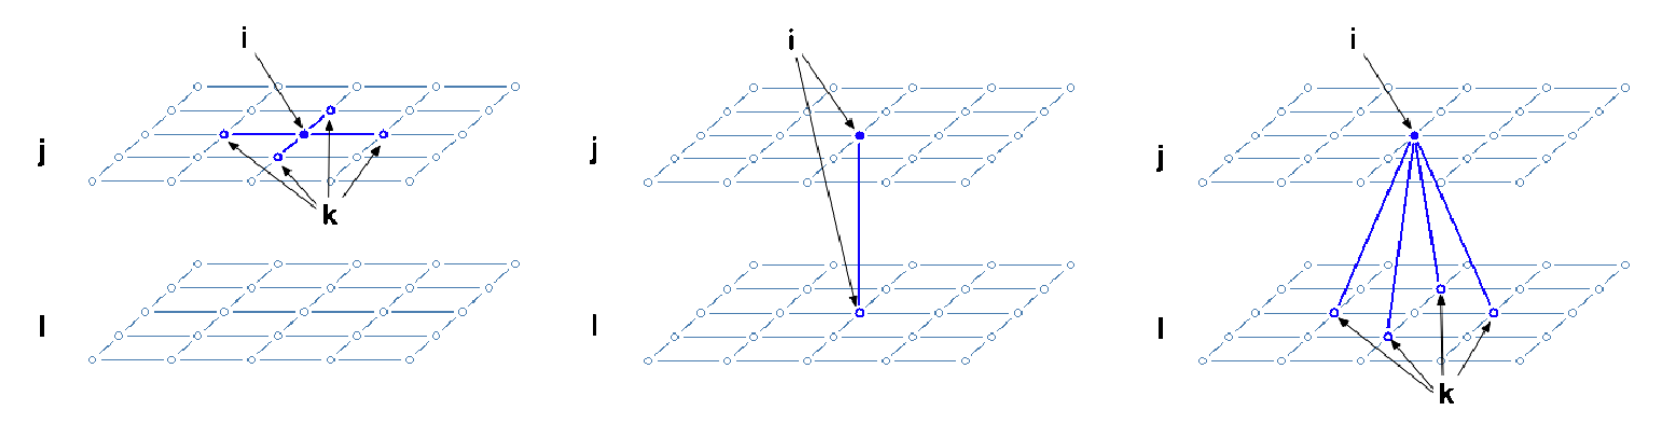
\includegraphics[width = 0.8\textwidth]{neighborhoods.png}}
  \caption{\small \emph{Examples of different types of neighborhoods. The left frame shows a within-variable spatial neighborhood, while the middle frame shows a within-location neighborhood. The right frame demonstrates the neighborhood associated with cross-variable connections. (Plot \& caption retrieved from \cite{paper})}}
  \label{fig: neighborhoods}
\end{figure}

\subsubsection{The Joint Distribution}
The key feature of this alternative formulation of MRF is that it stills falls within the original univariate framework of \cite{besag}, and the conditional mean and variance can be expressed as follows:
$$E[y_{ij} | y_{-ij}] = \mu_{ij} + \sum_{k \neq i} b_{ijkj} (y_{kj}-\mu_{kj}) +  \sum_{\ell \neq j} b_{iji\ell} (y_{i \ell}-\mu_{i \ell}) + \sum_{k,\ell \neq i,j} b_{ijk\ell} (y_{k\ell}-\mu_{k\ell})$$
and
$$Var[y_{ij} | y_{-ij}] = \tau_{ij}^2,$$
for all lattice points $i = 1, \dots,n$ and variables $j = 1, \dots,p$. p in this context is 2 and n is the total number of observations. $i$ is the location of interest, $j$ and $\ell$ are two different lattices, i.e., represent different variables (temperature and precipitation), $k$ here represents neighbors of interest.

Notice that the conditional mean is composed of, from left to right, an overall mean, the contribution to mean made by within-variable neighbors, the contribution to mean made by cross-variable but within-location neighbors, and the contribution to mean made by cross-variable and cross-location neighbors.

Now, the joint distribution is Gaussian with an $np \times 1$ mean vector 
$\boldsymbol{\mu} = [\boldsymbol{\mu}_1' , \dots, \boldsymbol{\mu}_n']'$ where $\boldsymbol{\mu}_i = [\mu_{i1}, \dots, \mu_{ip}]'$ are $p \times 1$ mean vectors correspond to each i; 
and with an $np \times np$ covariance matrix given by
\begin{eqnarray*}
    \begin{bmatrix}
        \boldsymbol{A}_1 & \boldsymbol{B}_{12} \delta_{12} & \cdots & & \boldsymbol{B}_{1n}\delta_{1n} \\
        \boldsymbol{B}_{21}\delta_{21} & \boldsymbol{A}_2 & & & \vdots \\
        \vdots & & \ddots &  & \\
        & & & \boldsymbol{A}_{n-1} & \boldsymbol{B}_{n-1, n}\delta_{n-1, n} \\
        \boldsymbol{B}_{n1}\delta_{n1} & \cdots &  & \boldsymbol{B}_{n, n-1}\delta_{n, n-1} &  \boldsymbol{A}_n
    \end{bmatrix}^{-1} \boldsymbol{T},
\end{eqnarray*}
where $\delta_{ik}$ are assumed to be equal to $\delta_{ki}$ and  $\delta_{ik} = \delta_{ki} = 1$ if $k \sim i$ and 0 otherwise. 
Each $\boldsymbol{A}$ is a $p\times p$ matrix defined by
$$
    \boldsymbol{A}_i = \begin{bmatrix}
        1 &  & -b_{ijk\ell} \\
         & \ddots  &  \\
        -b_{i\ell ij} &  & 1 
    \end{bmatrix}
$$
and each $\boldsymbol{B}$ is also a $p\times p$ matrix defined by
$$
\boldsymbol{B}_{ik} = \begin{bmatrix}
        -b_{i1k1} &  & -b_{ijk\ell} \\
         & \ddots  &  \\
        -b_{i\ell kj} &  & -b_{ipkp}
    \end{bmatrix},
$$
where $-b_{iji\ell}$ and $-b_{i\ell ij}$ are arbitrary off-diagonal elements of $\boldsymbol{A}_i$, and $-b_{ijk\ell}$ and $-b_{i\ell kj}$ are arbitrary off-diagonal elements of $\boldsymbol{B}_{ik}$. Lastly, $\boldsymbol{T} = \text{diag}(\tau_{11}^2, \dots, \tau_{1p}^2, \dots, \tau_{n1}^2, \dots, \tau_{np}^2)$ with $\tau_{ij}^2 = \tau_{j}^2$ for each j since the variance are assumed to vary across variables but not across locations. 

\subsection{Hierarchical Model for the RCM Experiment}
Let the n-dimensional vector $\boldsymbol{y}_{rj}$ denote the output of an RCM, in particular, the $r$th ensemble member for the $j$th variable. Then the hierarchy has three levels: the first level is data model, which describes the distribution of the observations; the second level is the process model, which consists of two parts and will be discussed below; the final level is the parameter model, where the priors of the parameters are assigned.

\subsubsection{Data Model}
The data model assumes that $\boldsymbol{y}_{rj}, \, r =1, \dots,m,j =1, \dots,p$, are independent with
$$\boldsymbol{y}_{rj} | \boldsymbol{\alpha}_j, \, \boldsymbol{\beta}_{rj}, \boldsymbol{h}_{rj}, \sigma^2_j \sim N(\boldsymbol{X}_1 \boldsymbol{\alpha}_j + \boldsymbol{X}_2 \boldsymbol{\beta}_{rj} + \boldsymbol{h}_{rj}, \, \sigma_j \boldsymbol{I}),$$
where $m$ indicates the number of ensemble members and $p$ indicates the number of variables (in this context, 2). $\boldsymbol{X}_1 \boldsymbol{\alpha}_j$ describes the general trend that is within the $j$th variable and hence not affected by initial conditions (therefore common to all ensemble members); $\boldsymbol{X}_2 \boldsymbol{\beta}_{rj}$ is the ensemble-specific trend within the $j$th variable; $\boldsymbol{h}_{rj}$ represents the spatial random effects; and $\sigma_j$ represents the variable-specific variance.

\subsubsection{Process Model}
The process model consists of two parts. The first part assumes $[\boldsymbol{\beta}_{r1}',\dots,\boldsymbol{\beta}_{rp}']', \, r = 1, \dots, m$ to be independent with
$$  \left .
    \begin{pmatrix}
        \boldsymbol{\beta}_{r1} \\
        \vdots \\
        \boldsymbol{\beta}_{rp}
    \end{pmatrix}  \right \vert
    \begin{pmatrix}
        \boldsymbol{\beta}_{1} \\
        \vdots \\
        \boldsymbol{\beta}_{p}
    \end{pmatrix}, \quad \boldsymbol{\Sigma}_b \sim N \left(   
        \begin{pmatrix}
            \boldsymbol{\beta}_{1} \\
            \vdots \\
            \boldsymbol{\beta}_{p}
        \end{pmatrix}, \boldsymbol{\Sigma}_b
    \right),
$$
where $\boldsymbol{\Sigma}_b$ is a $pq \times pq$ covariance matrix with $p$ the number of variables and $q$ the number of columns of $\boldsymbol{X}_2$. This part links the random regression coefficients specific to each ensemble member.

The second part assumes $[\boldsymbol{h}_{r1}', \dots, \boldsymbol{h}_{rp}']', r = 1, \dots, m$ to be independent with 
$$
    \left .
    \begin{pmatrix}
        \boldsymbol{h}_{r1} \\
        \vdots \\
        \boldsymbol{h}_{rp}
    \end{pmatrix}  \right \vert
    \begin{pmatrix}
        \boldsymbol{h}_{1} \\
        \vdots \\
        \boldsymbol{h}_{p}
    \end{pmatrix}, \quad \{\tau_j^2\}, \{\rho_{j\ell}\}, \{\phi_{j\ell}\} \sim N \left(   
        \begin{pmatrix}
            \boldsymbol{h}_{1} \\
            \vdots \\
            \boldsymbol{h}_{p}
        \end{pmatrix}, \boldsymbol{V}(\{\tau_j^2\}, \{\rho_{j\ell}\}, \{\phi_{j\ell}\})
    \right).
$$
The covariance matrix $\boldsymbol{V}$ is a function of three sets of independent parameters that describe variable specific variances, within-location dependencies, and cross-location dependencies correspondingly. The exact definition of these parameters will be provided in the next section. This part of the process model imposes a multivariate structure on the spatial random effects. The two parts in the process model are assumed to be independent. 

\subsubsection{Parameter Model}
The parameter model assumes priors of the following sets of parameters: 
\begin{itemize}
    \item the coefficients of trends, spatial random effects, and variable-specific variance: $\{\sigma_j \}, \{\boldsymbol{\alpha}_j \}, \{\boldsymbol{\beta}_j \}, \{\boldsymbol{h}_j\}, \boldsymbol{\Sigma}_b$
    \item the spatial dependencies: $\{\tau_j^2\}, \{\rho_{j\ell}\}, \{\phi_{j\ell}\}$
\end{itemize} 
In particular, $\rho_{j\ell}$ represents the cross-variable but within-location dependencies and $\phi_{j\ell}$ represents the cross-location dependencies, with $j = \ell$ meaning within-variable dependencies and $j \ne \ell$ meaning cross-variable and cross-location dependencies. 

\subsection{Posterior Distribution}
The posterior distribution, then, is given by Bayes Theorem as the following:
\begin{eqnarray*}
    P(\{\sigma_j \}, \{\boldsymbol{\alpha}_j \}, \{\boldsymbol{\beta}_{rj} \}, \{\boldsymbol{\beta}_{j} \} ,  \{\boldsymbol{h}_{rj}\}, \{\boldsymbol{h}_{j}\}, \boldsymbol{\Sigma}_b, \{\tau_j^2\}, \{\rho_{j\ell}\}, \{\phi_{j\ell}\}) | \boldsymbol{Y} \\
    \propto P(\boldsymbol{Y} | \{\sigma_j \}, \{\boldsymbol{\alpha}_j \}, \{\boldsymbol{\beta}_{rj} \}, \{\boldsymbol{h}_{rj}\}) \\
    \times P(\{\boldsymbol{\beta}_{rj}\} |  \{\boldsymbol{\beta}_j \}, \boldsymbol{\Sigma}_b) P(\{\boldsymbol{h}_{rj}\} | \{\boldsymbol{h}_j \}, \{\tau^2_j \}, \{\rho_{j\ell} \}, \{\phi_{j\ell}\}) \\
    \times P(\{\sigma_j \})P(\{\boldsymbol{\alpha}_j \})P(\{\boldsymbol{\beta}_j \}) P(\{\boldsymbol{h}_j\}) P(\boldsymbol{\Sigma}_b) P(\{\tau_j^2\}) P(\{\rho_{j\ell}\}, \{\phi_{j\ell}\}).
\end{eqnarray*}
There's no reason to assume the existence of a closed-form. \cite{paper} used Markov Chain Monte Carlo (MCMC) to sample from the posterior distribution; in particular, \cite{paper} implemented a Gibbs sampler and Metropolis-Hastings steps while needed. The speed is largely improved by the choice of an MRF model, for that the specification of an MRF involves precision matrix, which is largely sparse. Sparse Cholesky Decomposition was used extensively when implementing the Gibbs sampler for the MRF.


\section{Model Specification}
\subsection{Covariates}
In this experiment, there are $n = 44 \times 56 = 2464$ grid boxes in total. The number of variables $p = 2$, stands for temperature and total precipitation. The number of ensemble members $m = 3$ means three distinct set of initial conditions were used.

After some exploratory analysis done by \cite{paper}, (scaled) latitude, longitude, and elevation are used as covariates in the general trend (regression) component $\boldsymbol{X}_1 \boldsymbol{\alpha}_j$, to which an ensemble-specific trend random intercept $\boldsymbol{X}_2 \boldsymbol{\beta}_{rj}$ was added.
In addition, $\boldsymbol{\Sigma}_b$ was assumed to be of the form $\boldsymbol{\Sigma}_b = \sigma_{b}^2 I_{p}$ and $\rho_{j\ell}$ are assumed to be equal to a single constant $\rho$ since only two lattices were used in this experiment.

\subsection{Prior Selection}
\label{sec: priors}
The prior distributions assigned to the parameters are vague or noninformative because previous attempts to use informative priors largely yield biased results: 
\begin{eqnarray*}
    P(\sigma^2) &\propto& 1/\sigma^2 \text{ for } \sigma_{j}^2 \text{ and } \sigma_{b}^2\\
    \boldsymbol{\alpha}_j, \boldsymbol{h}_j &\sim& \mathcal{N}(\boldsymbol{0}, 10 \boldsymbol{I}_p) \\
    \boldsymbol{\beta}_j &\sim& \mathcal{N}(\boldsymbol{0}, 100 \boldsymbol{I}_p) \\
    \rho, \phi_{11}, \phi_{12}, \phi_{21}, \phi_{22} &\sim& Unif(\text{region of values that gives a positive definite covariance matrix})
\end{eqnarray*}
In particular, the region of values that gives a positive definite covariance matrix is identified by \cite{paper} used rejection sampling based on a sparse Cholesky Decomposition. Uniform distribution was chosen because any kind of concentrating priors at some sub-region will lead to biased estimates. 

\section{Results}
In the experiment conducted in \cite{paper}, the average temperature and average total precipitation of the winter season (December, January, and February) in a twenty-year window were computed, for both three control runs and three future runs for each of the $2464$ grid boxes. For each grid box, the differences between the control runs and future runs were also computed and recorded as the change in temperature and the change in total precipitation. Similarly, the differences for the summer season (June, July, and August) were also computed using the same approach. Visual representations of the computed differences are shown in Figure \ref{fig: Fig5} and Figure \ref{fig: Fig10} in the latter sections.

With the priors distributions discussed in section \ref{sec: priors}, an MCMC algorithm was used to obtain the posterior distributions of the conditional-dependence parameters. Gibbs sampler was implemented, and the parameters were updated using the Metropolis-Hastings algorithm. 

\begin{figure}
  \centering
   \fbox{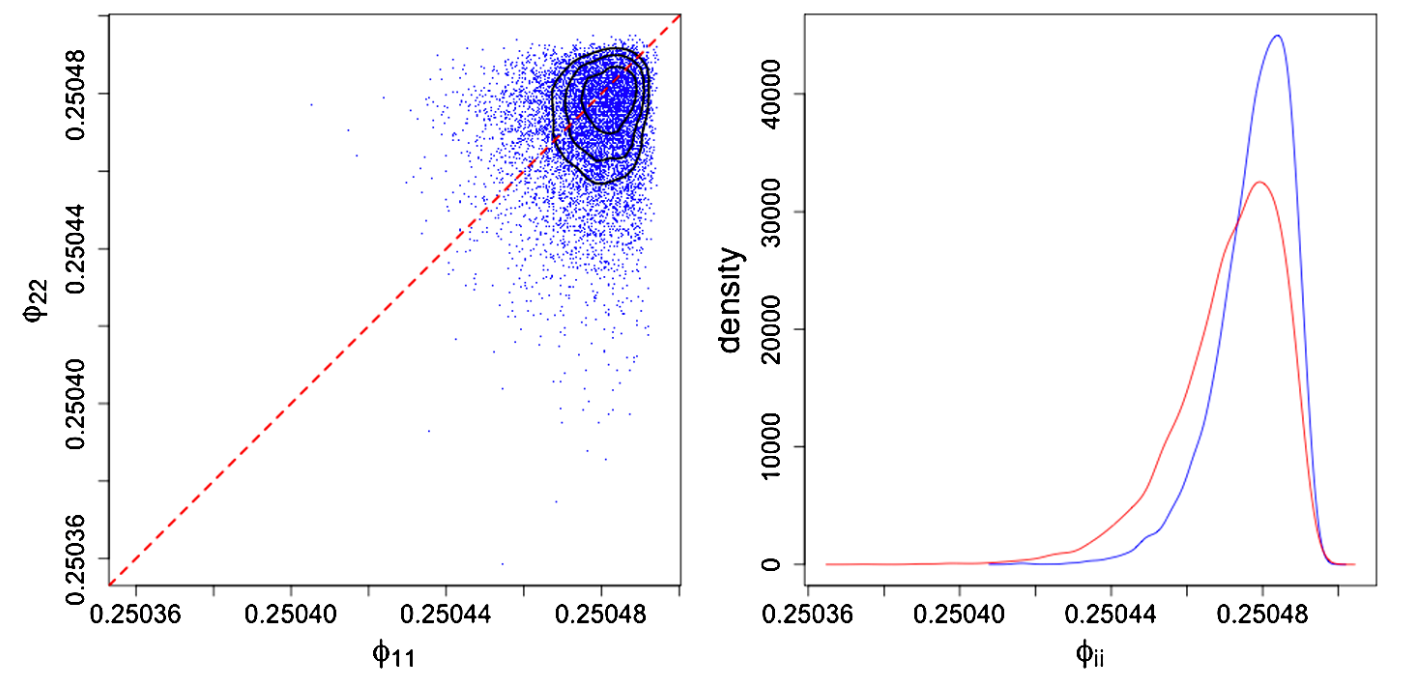
\includegraphics[width = 0.8\textwidth]{Fig3.png}}
  \caption{\small \emph{Left frame shows scatterplot of a random sample of 10,000 values of $\phi_{11}$ and $\phi_{22}$. Contours represent approximate 25, 50, and 75\% contours of a kernel density estimate. Right frame shows kernel density estimates of the marginals for $\phi_{11}$ (blue) and $\phi_{22}$ (red). (Plot \& caption retrieved from \cite{paper})}}
  \label{fig: Fig3}
\end{figure}

\subsection{Winter}
\subsubsection{Sampling Regime}
\label{sec: regimes}
The Gibbs sampling for winter contains three consecutive, one-after-another regimes. In the first regime, 2500 iterations were run, and each conditional-dependence parameter was updated one at a time. The purpose of this regime is to narrow down each conditional-dependence parameter to a reasonable range so that the burnin region would not be too long during sampling. 

The second regime has 10,000 iterations. In this regime, $\rho, \phi_{12}$, and $\phi_{21}$ were updated simultaneously, while $\phi_{11}$ and $\phi_{22}$ were still updated one at a time. In order to achieve an approximate $20 \%$ acceptance rate, the variance and the covariance matrix in the first and second regimes were updated periodically. The goal of this regime is to take extra care on the convergence of the conditional dependency parameters. As mentioned by \cite{paper}, posterior distributions of $\rho, \phi_{12}$, and $\phi_{21}$ converges after around 10,000 iterations, which corresponds to the end of the second regime. 

Similar to the second regime, the third regime also has 10,000 iterations, with the parameters being updated in the same approach. The only difference between the second and the third regime is that the proposal distribution is no longer being updated in the third regime. This last regime was designed to ensure the convergence of the posterior distributions of all parameters. Lastly, samples were obtained from the third regime to estimate the posterior distributions.  

\subsubsection{Estimates for Parameters}
\label{sec: WinParams}
In order to estimate the posterior distributions, 10,000 values of each parameter were sampled from the third regime, and the scatterplots of the samples and kernel estimates of the distributions are shown in Figure \ref{fig: Fig3} and Figure \ref{fig: Fig4}. 

Note that the points in the scatterplot in Figure \ref{fig: Fig3} are gathered around the positive boundary of positive values of $\phi_{11}$ and $\phi_{22}$, which suggests that both variables are conditionally spatial dependent within layer. That is, the temperature and precipitation of a given location depends considerably on the temperature and precipitation of its neighbors, respectively. Moreover, the plot of kernel density estimates demonstrated that the distribution of $\phi_{11}$ is tighter than that of $\phi_{22}$. While Both distributions centered around $0.25$, $\phi_{11}$ is more concentrated at this point, with a lower variance. Hence if we construct confidence intervals for these two parameters, the interval for $\phi_{11}$ should be narrower. 

A strong correlation between $\phi_{12}$ and $\phi_{21}$ is shown in Figure \ref{fig: Fig4}. In the scatterplot, most of the points are above the $45 ^\circ$ line. Furthermore, the plot of kernel density estimates also suggests that $\phi_{12}$ has a generally higher magnitude than $\phi_{21}$. Although the two distributions have similar shapes, the one for $\phi_{12}$ shifts to the right slightly, leading to a higher mean. Both plots provide evidence that for a given location, the conditional dependence between its temperature and neighboring total precipitation is stronger than the conditional dependence between its total precipitation and neighboring temperature. 

It is also worth noting that, according to \cite{paper}, almost all other published works involving the multivariate MRF models assume $\phi_{12} = \phi_{21}$, while the inference of the posterior distributions in \cite{paper} showed that this assumption is not appropriate in this case.

\begin{figure}
  \centering
   \fbox{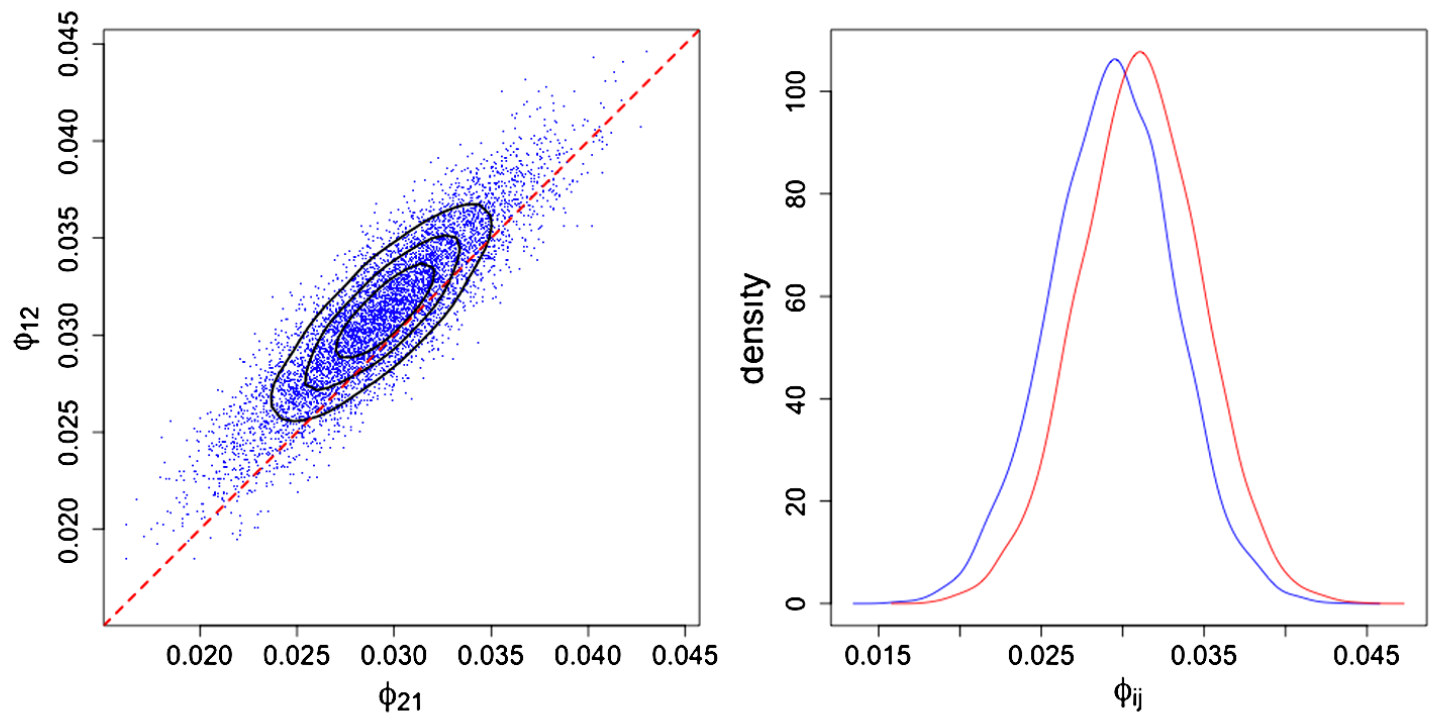
\includegraphics[width = 0.8\textwidth]{Fig4.png}}
  \caption{\small \emph{Left frame shows scatterplot of a random sample of 10,000 values of $\phi_{12}$ and $\phi_{21}$. Contours represent approximate 25, 50, and 75\% contours of a kernel density estimate. Right frame shows kernel density estimates of the marginals for $\phi_{12}$ (red) and $\phi_{21}$ (blue). (Plot \& caption retrieved from \cite{paper})}}
  \label{fig: Fig4}
\end{figure}

Lastly, according to \cite{paper}, the estimated posterior mean for $\rho$ is $-0.12$, and the estimated posterior standard deviation is $0.0014$. The negative value of the posterior mean suggests that the change in temperature is negatively correlated with the change in total precipitation. 

Figure \ref{fig: Fig7} shows the estimated probabilities of temperature increase, total precipitation decrease, and both at the same time, from left to right. This plot again provides evidence that increasing temperature and decreasing total precipitation are strongly associated, especially in the western coast. 

The posterior means for fixed and spatial effects for the differences between control runs and future runs are shown in Figure \ref{fig: Fig5}. This figure provides further evidence of Winter warming and decreasing total precipitation across the western US. 

\begin{figure}
  \centering
   \fbox{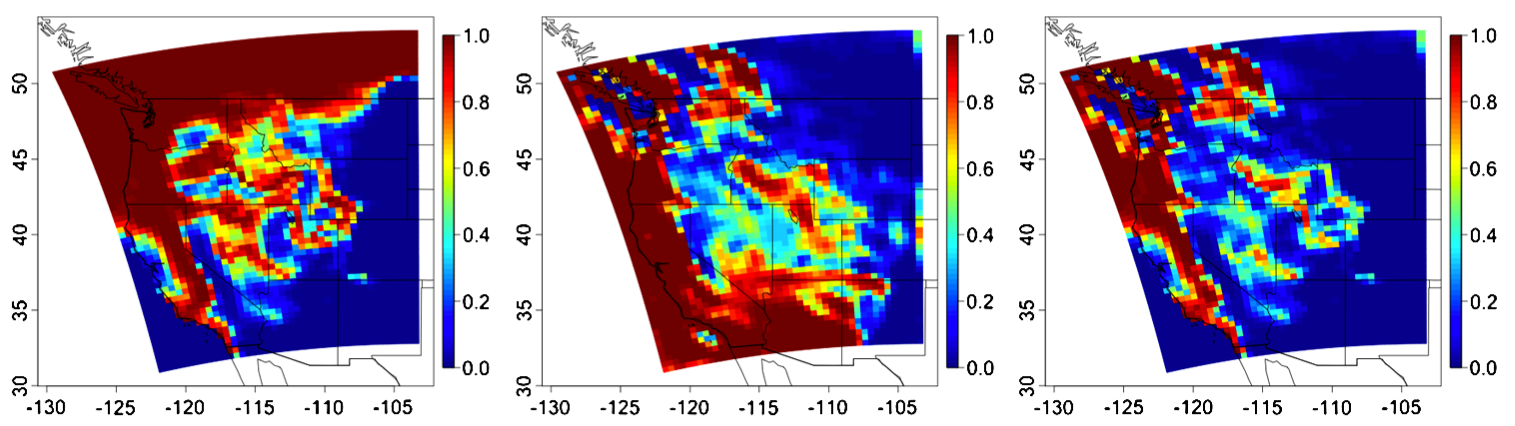
\includegraphics[width = 1\textwidth]{Fig7.png}}
  \caption{\small \emph{Estimated pointwise probabilities for the winter season: increasing temperature (left), decreasing total precipitation (middle), and simultaneously increasing temperature and decreasing total precipitation (right). (Plot \& caption retrieved from \cite{paper})}}
  \label{fig: Fig7}
\end{figure}

\begin{figure}
  \centering
   \fbox{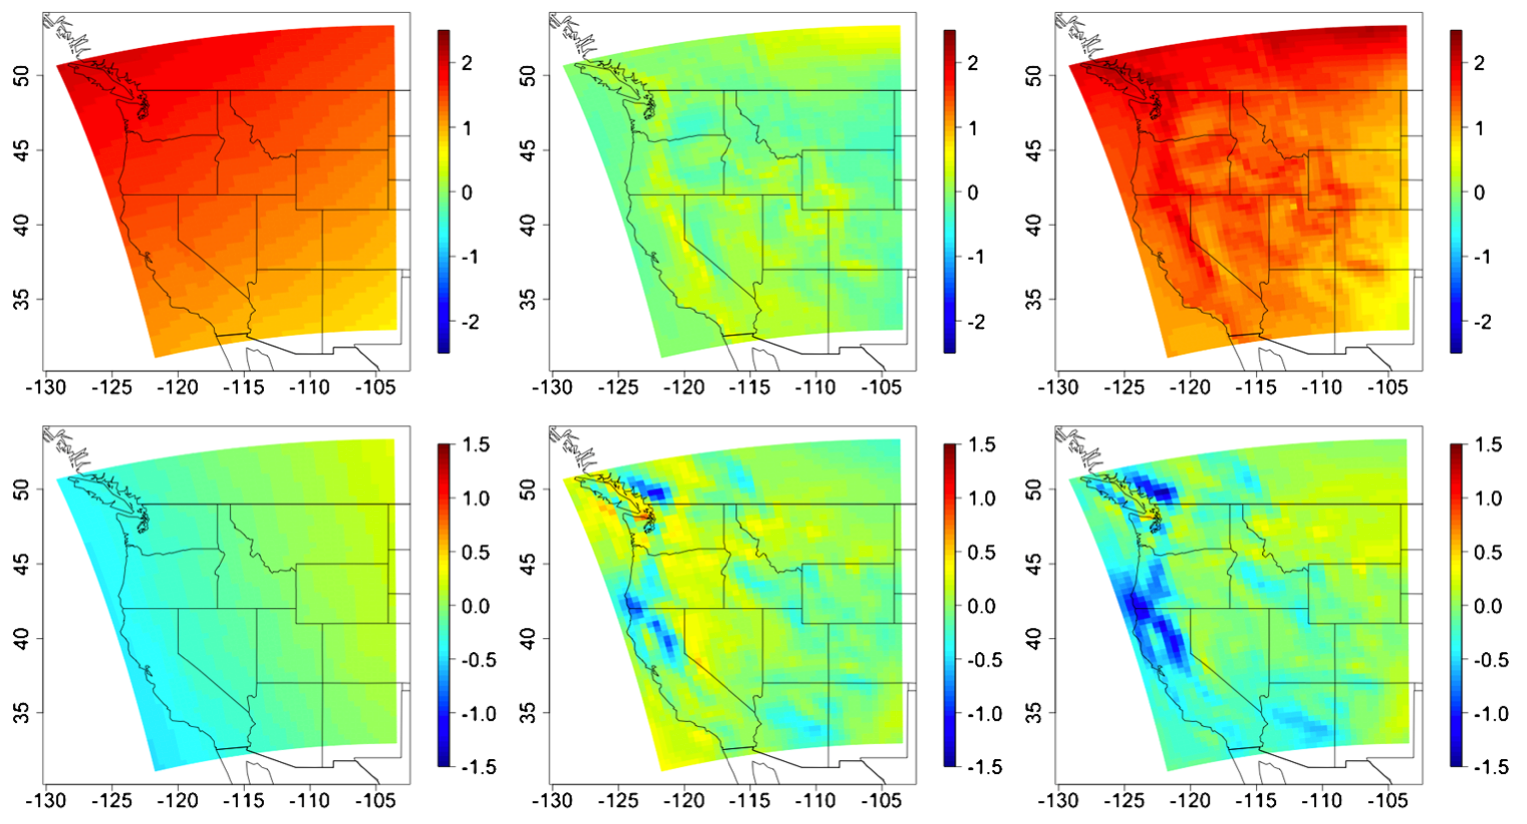
\includegraphics[width = 0.8\textwidth]{Fig5.png}}
  \caption{\small \emph{Posterior means for the regression (left), the spatial effect (middle), and the sum (right) for the winter season. The top row represents the change in midpoint temperature ($^\circ$K), while the bottom represents the change in total precipitation (inches). (Plot \& caption retrieved from \cite{paper})}}
  \label{fig: Fig5}
\end{figure}

\subsection{Summer}
\subsubsection{Sampling Regime}
The Gibbs sampler for summer follows a similar structure. Same as for winter, 2500 iterations were run in the first regime, with each conditional-dependence parameter being updated one at a time. 

The second regime is slightly different. Instead of 10,000 iterations, 20,000 iterations were run in this regime for summer. In addition, all five conditional-dependence parameters were updated simultaneously, instead of only three of them. The reason why the number of iterations was doubled is, as stated in \cite{paper}, it takes longer for the posterior distributions to converge. Consider the setting of the experiment, that no further updates to the proposed distribution were made in the third regime, it is crucial to observe convergence in distributions by the end of the second regime. Therefore, the number of iterations in the second regime should be big enough for the distributions to converge. For these reasons, although it is not mentioned in \cite{paper}, it is plausible to conclude that for the summer season, the distributions converge within 22,500 iterations.

Similar to the second regime, all five parameters were again updated simultaneously in the third regime. Same as for winter, the third regime contains 10,000 iterations, and the proposal distribution is no longer being updated. Samples were also obtained from this regime.  

\subsubsection{Estimates of Parameters}
\label{sec: SumParams}
The posterior distributions for parameters $\phi_{11}, \phi_{22}, \phi_{12}$, and $\phi_{21}$ are similar to that for the winter season, so we can still refer to Figure \ref{fig: Fig3} and Figure \ref{fig: Fig4} for their distributions. The only exception is $\rho$. For the summer season, the estimated posterior mean for $\rho$ is $-0.41$. Compare with the value of $-0.12$ \cite{paper} obtained for the winter season, it is plausible to say that the negative correlation between change in temperature and change in precipitation in the summer is stronger than that in the winter. 

Similar to Figure \ref{fig: Fig7}, Figure \ref{fig: Fig12} also shows the same probabilities for the summer season. Note that the increasing temperature and decreasing total precipitation in summer is more widespread, and focus more on the eastern side.

\begin{figure}
  \centering
   \fbox{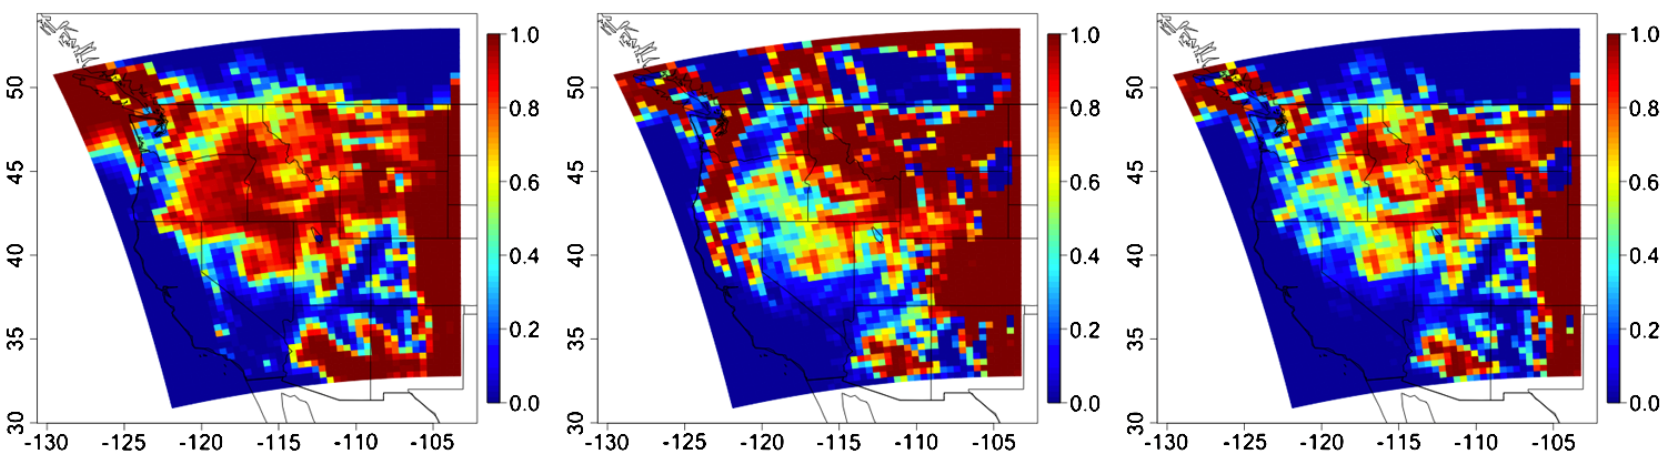
\includegraphics[width = 1\textwidth]{Fig12.png}}
  \caption{\small \emph{Estimated pointwise probabilities for the summer season: increasing temperature (left), decreasing total precipitation (middle), and simultaneously increasing temperature and decreasing total precipitation (right). (Plot \& caption retrieved from \cite{paper})}}
  \label{fig: Fig12}
\end{figure}

The effects for change in temperature and total precipitation for the summer precipitation is shown in Figure \ref{fig: Fig10}. Again, this plot provides evidence of summer warming and decreasing in total precipitation focusing in the eastern side of the domain.

\begin{figure}
  \centering
   \fbox{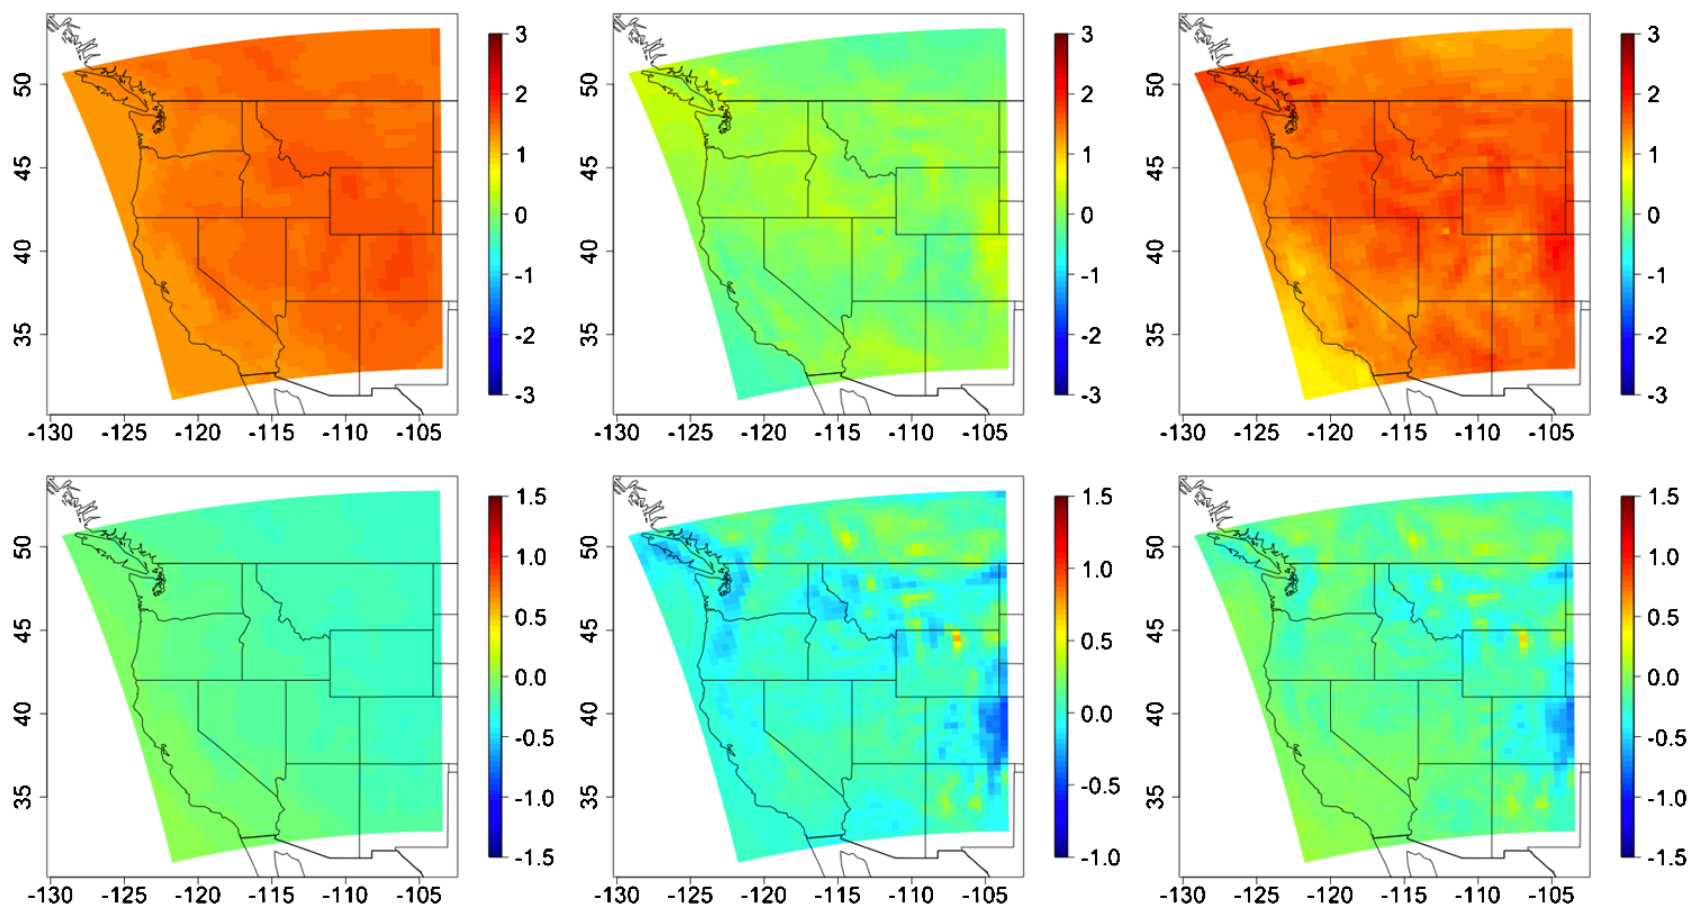
\includegraphics[width = 0.8\textwidth]{Fig10.png}}
  \caption{\small \emph{Posterior means for the regression (left), the spatial effect (middle), and the sum (right) for the summer season. The top row represents the change in midpoint temperature ($^\circ$K), while the bottom represents the change in total precipitation (inches). (Plot \& caption retrieved from \cite{paper})}}
  \label{fig: Fig10}
\end{figure}

\section{Conclusion}
In order to better study climate and climate change, it is important to study and quantify the uncertainty in the climate-model output. And due to the limitations on the number of runs that can be produced, statistical models become necessary in order to quantify the output distribution, as well as the breadth of variation in the model output. However, various challenges has been posted in the path of developing a good model. The conventional challenges include:
\begin{itemize}
    \item Difficulty when trying to accurately reflect the change in certain aspects (variables) of climate
    \item Model the data of more than 1 variables simultaneously
    \item Extremely high computational cost while trying to model more than 1 variables
\end{itemize}

 The first several decades of attempts by climatologists and geostatisticians in trying to represent the climate system as truthfully as possible used full Gaussian Spatial Process models. However, the full Gaussian Spatial Process models are so computationally expensive that it could take weeks or even months to estimate one set of parameters. This challenge was effectively tackled after the basic framework of MRF models was laid out by \cite{besag}. The key feature was that the observation at one spatial location can be expressed by a linear combination of the observations in neighboring locations. This hugely reduced computational cost.

Shortly after the first challenge was solved, a second challenge follows: climatologists and geostatisticians now want to model the data of more than one variable at the same time. Previous models only have one observation at a spatial lattice point, how could they be modified to include more? \cite{mardia} managed to make a progress by updating the CAR framework via extending the univariate structure to multivariate structure. Then, multiple observations were allowed at a single spatial lattice point. However, that model was extremely difficult to implement without dramatic simplification or use of restrictive priors. To come up with a solution that allows simultaneous modeling of the data of more than 1 variables while keeping the computation cost low, \cite{paper} introduced an alternative formulation of multivariate MRF. The core idea involves a stacking of lattices. This formulation still falls within the original univariate CAR framework, but there's no restriction on the number of variables that can be modeled. 

The last challenge arises when sampling from a very complex posterior distribution with no close form. Typically with MRFs, sparse Cholesky decomposition would be extensively used with MCMC to sample from the posterior distribution due to the fact that the precision matrices in MRFs are usually very sparse. But besides the computational advantages brought by MRFs, \cite{paper} used a package called \texttt{spam} developed by themselves to bypass the typical three-step-procedure involved in sparse Cholesky decomposition. This took the computational efficiency to a whole new level. 

In conclusion, \cite{paper} successfully developed a hierarchical spatial statistical method that can quantify the probabilistic projections and the correlation between fields and joint projections of the outputs from regional climate model ensembles. \cite{paper} is the first using the hierarchical approach to perform \emph{spatial analysis} of \emph{multivariate} output from RCMs. \cite{paper} also contributes to a growing collection of studies that focus on modeling asymmetric cross-dependence structures for multivariate spatial data.

\section{Discussion}
The innovative way of representing multivariate lattice data implemented by \cite{paper} raised a great computational benefit and improved model flexibility. Number of variables could easily be added through stacking one additional lattice; number of sets of initial conditions could be easily increased by adding a member in the ensemble; besides, the range of neighbors can also be extended for better prediction accuracy while needed. Moreover, more predictors based on climatology can be added outside longitude, latitude, and elevation. However, addition of extra variable, ensemble member, neighbor, or predictor would perforce lead to increase in complexity of the model and hence computational cost. The trade-off must be examined closely before making any decisions. 

The result of \cite{paper} is conditional on the initial conditions, including initial states of the climate, assumption of initial forcings, and understanding of the physical processes, that are inherent to the particular regional climate model. Unreasonable generalizations shall not be made casually.

Several confusing notations and omissions of explanation can be spotted in  \cite{paper}. First of all, $\boldsymbol{X}_1$ and $\boldsymbol{X}_2$ that first appeared in the formulation of hierarchical model is a little bit confusing. The intuition was that these two matrices represent general trend and ensemble-specific trend, correspondingly; but what exactly is $\boldsymbol{X}_1$ and $\boldsymbol{X}_2$? No explanation was provided. 

Secondly, there was no formal definition of $\rho, \phi_{11}, \phi_{12}, \phi_{21}, \phi_{22}$. Readers have to cross compare the text description of some of them with the graphs provided in the result section to come up with a guess of what each of them means. 

Thirdly, the reason why, unlike the winter sampling regimes, the second regime of summer sampling regimes have 20000 runs is not explained. Indeed it was because it took longer for all the parameters to converge, but why? One could argue that it was because all five parameters were being updated simultaneously instead just three of them, but again the reason was not mentioned. What is the difference between summer and winter? Why different sampling regimes were used? These questions, if answered, will be very conducive for the readers to interpret. 

\bibliographystyle{apalike} 
\bibliography{References.bib} 

\end{document}